\section{系统设计}

\subsection{体系结构概览}

EdgeSched 采用分层架构设计，如图~\ref{fig:architecture} 所示。系统自上而下分为表示层、领域层、控制平面、执行层和数据适配层。用户请求通过 WebSocket 接口进入系统，由领域层业务逻辑处理，再由控制平面统一路由到相应的执行组件。

\begin{figure}[!t]
\centering
\IfFileExists{figures/diagrams/system_architecture.pdf}{%
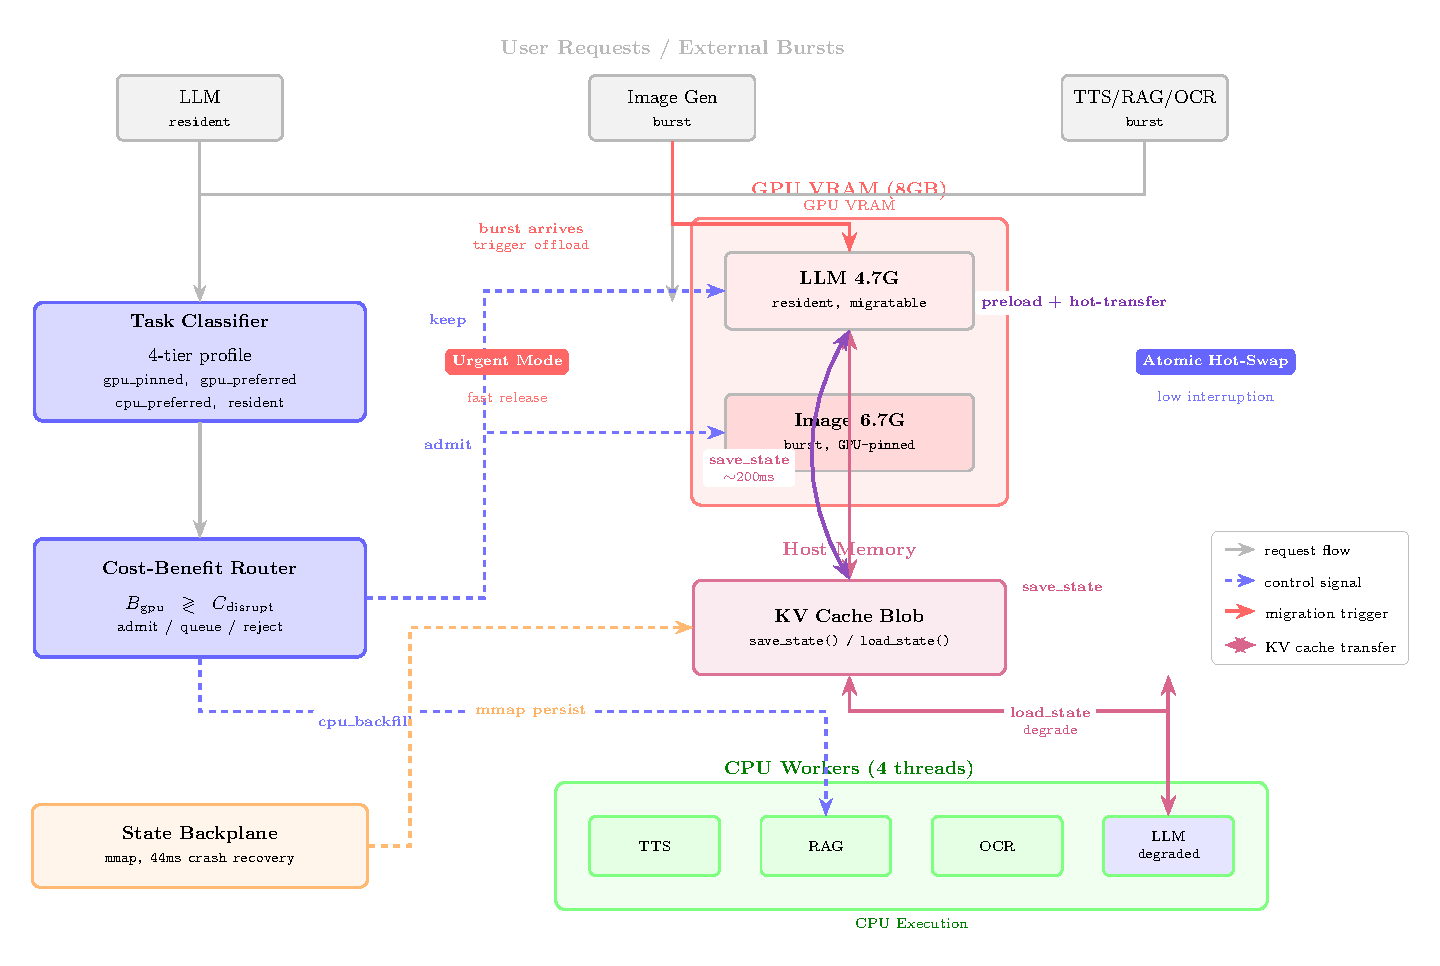
\includegraphics[width=0.95\columnwidth]{figures/diagrams/system_architecture.pdf}%
}{%
\fbox{\parbox{0.92\columnwidth}{\centering 当前工作区构建中缺少系统架构图。}}%
}
\caption{EdgeSched 的分层系统架构。控制平面负责任务路由与编排，执行平面负责 GPU/CPU 资源迁移。}
\label{fig:architecture}
\end{figure}

控制平面包含三个核心组件：
\begin{enumerate}
\item \textbf{GlobalTaskScheduler} 作为 L1 路由层，负责任务分发、优先级队列管理、取消事件以及图像任务的反压控制。
\item \textbf{CPPSchedulerEngine} 作为 L2 高性能执行层，封装 llama-cpp-python 推理引擎，并实现 GPU/CPU 动态资源迁移。
\item \textbf{StateBackplane} 基于 mmap 实现零拷贝状态持久化，支持在崩溃后约 44 ms 内恢复到语义上可用的任务状态。
\end{enumerate}

执行层包含 \texttt{ResourceManager}，负责协调模型生命周期和 GPU/CPU 资源分配，并在多个模型之间仲裁资源竞争。数据适配层包含 LLM Adapter 和 Image Adapter，分别封装大语言模型（GGUF 格式）与图像生成模型（Stable Diffusion）的推理逻辑，以屏蔽底层推理引擎差异，并支持多个后端之间的无缝切换。

\subsection{双任务调度}

EdgeSched 将第 2 节介绍的场景具体化为本地 AI 运行时中一对冲突强烈的工作负载：常驻、交互式、可迁移的 LLM 服务，以及突发、GPU 绑定的图像生成任务。前者即使在临时降级时也应保持可达，后者则可以排队，但必须在可接受时延内通过独占 GPU 完成。

因此，调度器对这两类任务采用不同处理方式。LLM 任务通过 \texttt{submit\_llm\_task()} 直接提交给 CPPSchedulerEngine，默认占用 GPU 以维持低延迟。图像生成任务则通过 \texttt{try\_enqueue\_image\_generation()} 进入独立的有界队列。当图像任务到来而 LLM 正占用 GPU 显存时，调度器会触发资源迁移，使常驻任务降级到 CPU 执行，并让突发任务获得独占 GPU 访问权。如果多个图像任务连续到达，后续任务继续排队；当队列已满时，反压机制会拒绝新任务，以避免资源耗尽和系统行为不稳定。算法~\ref{alg:scheduling} 给出了核心调度逻辑。

\begin{algorithm}[!t]
\caption{带反压的任务调度}
\label{alg:scheduling}
\begin{algorithmic}[1]
\STATE \textbf{function} \textsc{SubmitTask}(task)
\IF{task.type == LLM}
    \STATE Submit to CPPSchedulerEngine
    \STATE Allocate GPU by default
\ELSIF{task.type == IMAGE}
    \IF{queue.size() $<$ total\_slots}
        \STATE Enqueue task
        \IF{LLM is on GPU}
            \STATE Trigger \textsc{OffloadToCPU}()
        \ENDIF
    \ELSE
        \STATE \textbf{throw} QueueFullError
    \ENDIF
\ENDIF
\STATE \textbf{end function}
\end{algorithmic}
\end{algorithm}

这种设计的目标，是在为突发任务提供可预测资源分配的同时，尽量保持常驻服务的可用性。

设计意图并不只是“让某个队列优先级更高”。更准确地说，调度器认为这两种角色承担着不同义务：常驻服务在竞争全过程中都应保持可达，而突发任务则可以等待，但一旦被接纳就应获得独占 GPU 所有权。后续控制逻辑都由这一观察出发。

\subsection{不对称迁移的设计动机}

EdgeSched 的关键观察是，两条迁移路径服务于不同的控制目标。当一个突发的 GPU 绑定任务到来时，系统面临硬性的显存压力：此时的直接目标是尽量缩短释放时间，以便在 OOM 发生前回收 GPU。在这个阶段，常驻任务短暂降级是可以接受的，而延迟释放 GPU 则不可接受。相对地，当突发任务完成、显存再次可用之后，首要目标不再是内存安全，而是恢复高性能推理时尽量减少用户可见中断。在这个阶段，保持服务连续性比追求最短原始重载时间更重要。

这种不对称意味着，单一的对称迁移流程不仅次优，而且从根本上无法同时优化两个方向。如果调度器针对快速释放进行调优，它就必须迅速中断并丢弃 GPU 执行上下文，这有利于 GPU$\rightarrow$CPU 路径，却会直接破坏恢复连续性；如果它针对无缝恢复进行调优，就必须后台预加载并延迟切换，这有利于 CPU$\rightarrow$GPU 路径，却会在竞争到来时延后显存回收。这两个要求因此天然相互张力：“快速释放”和“无中断恢复”不可能由同一个对称策略同时最优满足。GPU$\rightarrow$CPU 路径应优先追求快速释放显存和上下文保留，而 CPU$\rightarrow$GPU 路径应优先追求低中断恢复与延迟切换。因此，EdgeSched 在下行迁移中使用 \textbf{Urgent Mode}，在上行恢复中使用 \textbf{Atomic Hot-Swap}。

换句话说，EdgeSched 的新意并不在于优先级队列、模型卸载或状态恢复这些单个部件本身是新的；真正的主张是：在单台内存受限设备上，两条迁移方向必须受\emph{不同控制目标}支配，而这会带来无法回避的设计权衡。一个对称的重载流程不可能同时实现最快的安全下行与最少打扰的上行恢复；它必然要牺牲其中一个目标去换取另一个目标的改善。从这个意义上说，不对称性是工作负载约束的必然结果，而不是可选的工程润色。

\subsection{动态资源迁移}

图~\ref{fig:migration_flow} 展示了完整的资源迁移工作流。

\begin{figure}[!t]
\centering
\IfFileExists{figures/diagrams/migration_flow.pdf}{%
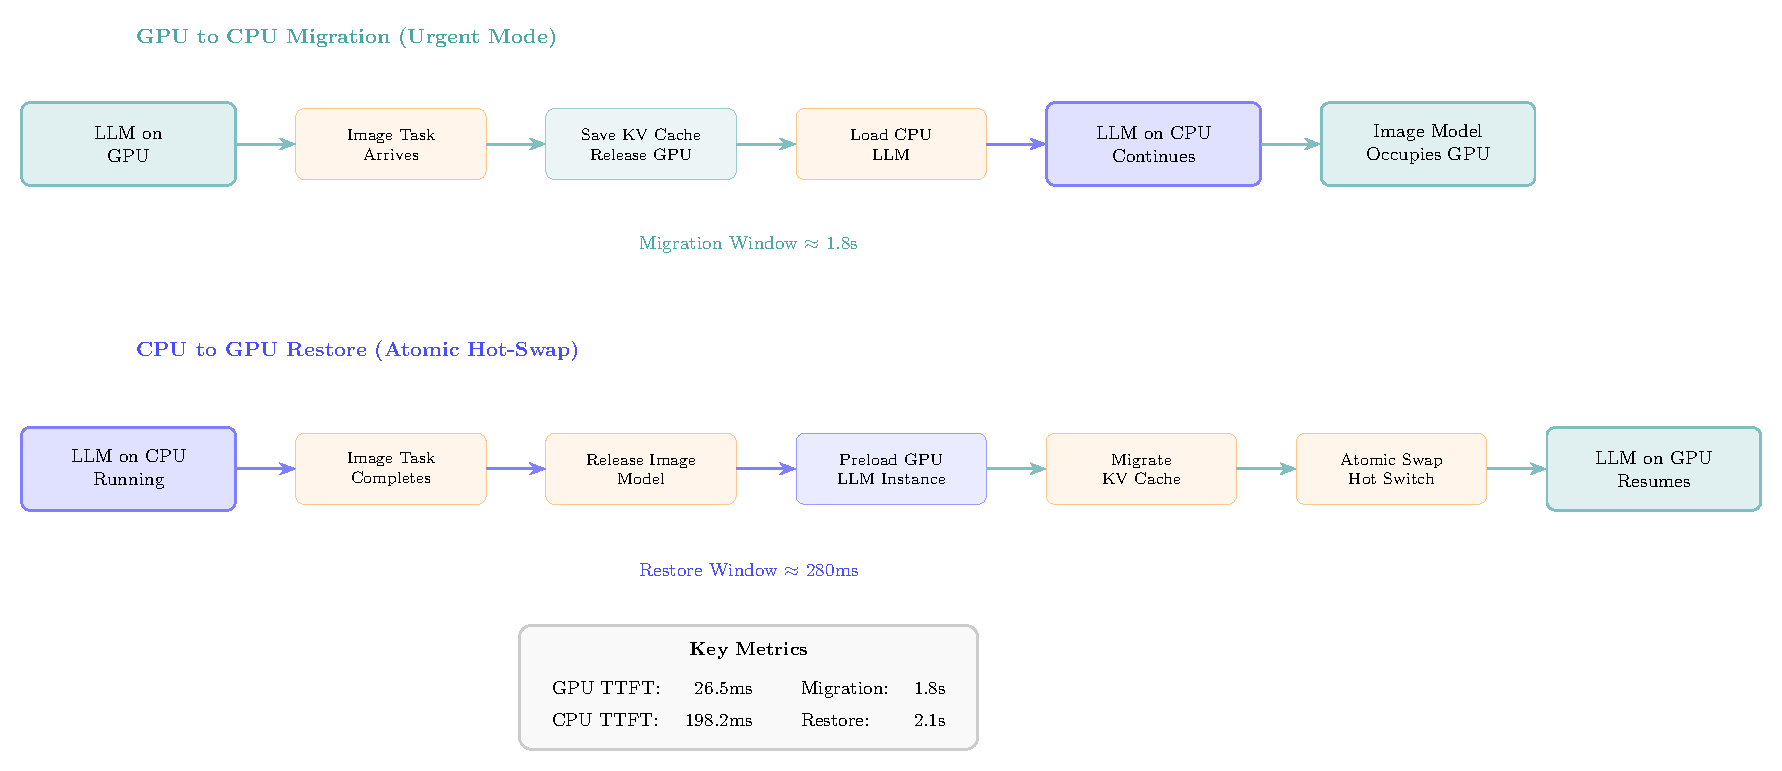
\includegraphics[width=0.95\columnwidth]{figures/diagrams/migration_flow.pdf}%
}{%
\fbox{\parbox{0.92\columnwidth}{\centering 当前工作区构建中缺少迁移流程图。}}%
}
\caption{资源迁移工作流，展示了不对称策略：用于快速抢占的 Urgent Mode（GPU$\rightarrow$CPU）和用于低中断恢复的 Atomic Hot-Swap（CPU$\rightarrow$GPU）。}
\label{fig:migration_flow}
\end{figure}

\subsubsection{不对称迁移策略}

\textbf{下行（GPU $\rightarrow$ CPU）：Urgent Mode}。当图像任务到来时，系统触发紧急迁移以快速释放显存。该策略针对内存安全进行优化：系统首先通过 \texttt{save\_state()} 将 KV cache 从显存复制到主机内存中（在我们的测量中约为 200--300 ms），以保留对话上下文；随后释放 GPU 分配，从而以较低 OOM 风险加载图像模型。释放完成后，系统并行启动两项操作：后台加载 CPU 版 LLM 实例（可受益于 OS 页缓存），以及将图像生成模型加载到 GPU。换言之，Urgent Mode 接受短暂的性能下降，以换取有界的释放时间。

\textbf{上行（CPU $\rightarrow$ GPU）：Atomic Hot-Swap}。当图像任务完成、显存重新可用时，系统执行原子热切换以恢复高性能 LLM 推理。该策略优化的是服务连续性，而不是立即完成切换。它采用双缓冲策略：
\begin{enumerate}
\item \textbf{预加载}：先在 GPU 上加载一个新的 LLM 实例，同时 CPU 实例继续处理用户请求。
\item \textbf{热迁移}：GPU 实例就绪后，短暂停顿 CPU 实例，通过 \texttt{save\_state()} 导出 KV cache，并将其加载到 GPU 实例中。
\item \textbf{切换与卸载}：最后原子替换活动实例指针，将新请求路由到 GPU 实例，并异步卸载 CPU 实例。
\end{enumerate}

在我们的实现中，这种模式将恢复过程中的用户可见中断限制在最终状态转移与切换窗口内，而不是完整的 GPU 重载时间。从概念上讲，这更接近预加载和延迟切换这类已有的高可用性技术，而不是声称发明了新的底层原语~\cite{cully2008remus}。EdgeSched 的贡献在于：只在上行路径应用这种面向连续性的策略，而在下行路径采用更激进的内存安全策略。

\subsubsection{实现机制}

不对称迁移的实现依赖三个核心机制：
\begin{enumerate}
\item \textbf{并发控制}：使用 \texttt{asyncio.Lock()} 保持实例替换的原子性，并降低竞态风险。
\item \textbf{状态序列化}：使用 llama-cpp-python 的 \texttt{save\_state()} / \texttt{load\_state()} 接口，在 GPU 支持和 CPU 支持的实例之间迁移 KV cache 状态。
\item \textbf{异步清理}：通过 \texttt{asyncio.create\_task()} 在后台释放旧实例，避免阻塞主服务路径。
\end{enumerate}

\subsection{反压控制}

图像生成任务计算开销高且显存占用大，因此系统采用有界队列来防止资源耗尽。图像队列容量由 \texttt{queue\_capacity}（默认 8）和 \texttt{max\_concurrent}（默认 1）共同决定，总槽位为二者之和（默认 9）。其中 \texttt{max\_concurrent} 表示并发执行数，\texttt{queue\_capacity} 表示排队等待数。

队列管理通过 \texttt{try\_enqueue\_image\_generation()} 实现：系统使用 \texttt{asyncio.Queue(maxsize=total\_slots)} 创建有界队列；若队列未满，则任务入队等待执行；若队列已满，则抛出 \texttt{RuntimeError("Image queue is full")} 拒绝请求。这种设计的目标是在高负载下保持系统行为可预测，而不是放任任务无限累积、进一步恶化内存压力和响应时延。

此外，系统还跟踪图像任务状态（pending/running/completed），支持任务取消和结果查询，并使任务生命周期状态对用户可见。

\subsection{取消语义}

系统支持用户主动取消正在执行或排队中的任务，并采用协作式中断策略以避免资源泄漏。

\textbf{LLM 流式取消}。LLM 生成采用流式输出，并通过 \texttt{asyncio.Event} 实现协作式取消。用户调用 \texttt{cancel\_llm\_request(request\_id)} 后，系统设置取消标记；生成循环在每个 token 后检查该标记，如已置位则停止后续生成。该模式避免了强制终止，并降低了资源泄漏风险。

\textbf{图像任务取消}。排队中的图像任务会被直接丢弃；执行中的任务只设置取消标记，但不能被强制中断，必须等待其执行完成。系统通过 \texttt{cancel\_image\_job(job\_id)} 接口提供取消能力；被取消任务的结果会被丢弃，不会推送给用户。

\textbf{局限性}。系统不支持硬中断（即强制杀死 GPU 任务），这受 CUDA 显存管理机制约束。运行中的图像任务必须等待完成；取消仅影响结果是否被推送。这一设计承认“不可硬中断”的边界，并在资源安全与响应速度之间做出平衡。

\subsection{崩溃恢复}

本地部署环境并不稳定，系统可能因断电或异常而崩溃。StateBackplane 基于 mmap 实现零拷贝状态持久化，其目标是在系统重启后约 44 ms 内把任务状态恢复到语义上可用的状态。

\textbf{数据布局}。持久化文件大小为 1MB，分为三个区域：Header（8B）存储 Magic Number 和版本号，用于数据完整性校验；Task Slots（32 个槽位，每个 48B）存储任务 ID、状态、优先级和时间戳；其余空间保留作扩展。

\textbf{持久化机制}。任务状态发生变化时，系统通过 \texttt{register\_task()} 和 \texttt{update\_task\_status()} 实时写入 mmap 文件。由于 mmap 直接将文件映射到内存地址空间，读写操作等价于内存访问，无需传统 I/O 的数据拷贝，时延仅为微秒级。

\textbf{恢复过程}。系统重启时，StateBackplane 在初始化阶段读取持久化文件：先验证 magic number 和版本号以确保数据格式正确；再遍历 32 个任务槽位，提取状态非零的活跃任务；将 Pending 状态任务重新加入调度队列；并把 Running 状态任务标记为 Failed，以避免留下悬挂任务。这一设计在崩溃后保留了可恢复的任务元数据，并提供了最低可行的任务闭环语义。算法~\ref{alg:recovery} 给出了恢复逻辑。

\begin{algorithm}[!t]
\caption{崩溃恢复流程}
\label{alg:recovery}
\begin{algorithmic}[1]
\STATE \textbf{function} \textsc{RecoverFromCrash}()
\STATE Open mmap file
\IF{magic\_number $\neq$ EXPECTED}
    \STATE \textbf{throw} CorruptedDataError
\ENDIF
\STATE recovered\_tasks $\leftarrow$ []
\FOR{slot in task\_slots[0:32]}
    \IF{slot.state $\neq$ EMPTY}
        \IF{slot.state == PENDING}
            \STATE Re-enqueue to scheduler
        \ELSIF{slot.state == RUNNING}
            \STATE Mark as FAILED
        \ENDIF
        \STATE recovered\_tasks.append(slot)
    \ENDIF
\ENDFOR
\STATE \textbf{return} recovered\_tasks
\STATE \textbf{end function}
\end{algorithmic}
\end{algorithm}